% 6 Results and lessons learned -- 2.75 pages (results ~2.0, lessons ~0.75)
\section{Results and Lessons Learned}
\label{sec:results}

\begin{table*}[t]
\centering
\caption{Detection on the bench's 504 graded answers per system (258 pairs $\times$ 2 wordings, without the 12 the trace cannot show). \sysname: run 1, and the mean $\pm$ standard deviation over three runs. ``Abstain'': share of answers that said ``cannot tell''. Cost: model API cost of the run's 516 answers at list price; \textsuperscript{*}\sysname's answer call only, as its skills' calls were not logged.}
\label{tab:main}
\small
\begin{tabular}{@{}lrrrrrrrrrrr@{}}
\toprule
System & TP & FN & FP & TN & Precision & Recall & Specificity & $F_1$ & Bal.\ acc. & Abstain & Cost (\$) \\
\midrule
LLM only & 42 & 106 & 42 & 314 & 0.50 & 0.28 & 0.88 & 0.36 & 0.58 & 72\% & 2.41 \\
RAG      & 41 & 107 & 40 & 316 & 0.51 & 0.28 & 0.89 & 0.36 & 0.58 & 70\% & 2.74 \\
TMLL     & 82 & 66 & 62 & 294 & 0.57 & 0.55 & 0.83 & 0.56 & 0.69 & 45\% & 8.63 \\
Codex    & 134 & 14 & 113 & 243 & 0.54 & 0.91 & 0.68 & 0.68 & 0.79 & 8\% & 9.50 \\
\midrule
\sysname (run 1) & 137 & 11 & 24 & 332 & 0.85 & 0.93 & 0.93 & 0.89 & \textbf{0.93} & 3\% & 1.41\textsuperscript{*} \\
\sysname (3 runs) & & & & & .854{\scriptsize$\pm$.007} & .926{\scriptsize$\pm$.007} & .934{\scriptsize$\pm$.003} & .889{\scriptsize$\pm$.007} & \textbf{.930}{\scriptsize$\pm$.005} & & \\
\bottomrule
\end{tabular}
\end{table*}

\subsection{RQ1: Accuracy}

Table~\ref{tab:main} gives the main result. \sysname reaches a balanced accuracy of 0.93, with recall 0.93 and specificity 0.93: it found 137 of the 148 present symptoms and reported 24 symptoms that were not there among 356 absent pairs. The best baseline, Codex, reaches 0.79. TMLL, which sees Trace Compass's analyses of the whole trace but nothing computed for the question, reaches 0.69. The two baselines that read trace text, LLM only and RAG, reach 0.58 each. Retrieval worked: the documents were mostly on topic (the critical path, thread states, runnable threads, CPU migration; 10\% were the Django distractors). But they explain concepts a current model already knows, while what it lacks is evidence, and the slice holds only a few milliseconds of every few seconds. Retrieval pays off for knowledge the model does not have, such as an organization's documentation of its own software. In our prototype study, adding retrieval with the same kind of document raised a trace-text baseline from 35\% to 68\%. That is the role of RAG in \sysname: bringing in internal documentation of the software being traced. The bench leaves such documents out so that its scores measure what each system reads from the trace. Codex, which can compute anything it chooses from the whole trace, found nearly as many symptoms as \sysname (recall 0.91 against 0.93) but also reported 113 symptoms that were not there, answering ``yes'' on 32\% of absent pairs (specificity 0.68).

\textbf{Example.} Fig.~\ref{fig:pipeline} follows one question: \emph{``Do two or more threads of batch\_server each hold a lock that another of them needs, so that they stay blocked for good?''}, asked of the trace where \texttt{worker-1} and \texttt{worker-3} deadlock 12\,s into the run. All four baselines answered ``cannot tell''. TMLL and Codex both named the right two threads as ``the strongest candidates'', from futex waits that persisted to the end of the trace, but did not commit. \sysname's stuck-wait detection reported that both threads entered lock-style futex waits on different addresses 2\,ms apart and were still blocked when the trace ended, 18.2\,s later, while the process made no further progress. It answered ``yes'', named both threads, and noted that a kernel trace cannot show which thread owns each lock, in 11\,s.

\subsection{RQ2: False Alarms and Abstention}

\begin{figure}[t]
\centering
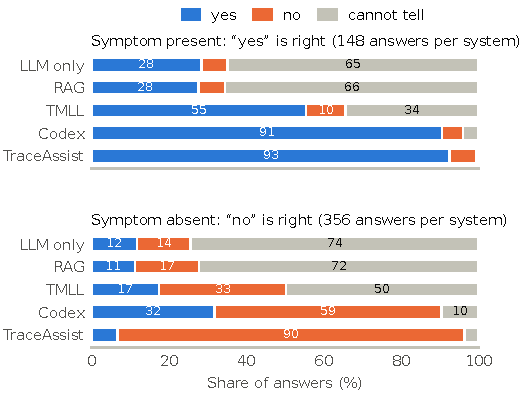
\includegraphics[width=\columnwidth]{verdicts}
\Description{Two panels of horizontal stacked bars, one per system, showing the share of yes, no and cannot-tell answers on present and on absent pairs.}
\caption{What each system answered (run 1, both wordings), as a share of its answers on pairs where the symptom is present (top) and absent (bottom). The text baselines mostly answer ``cannot tell''; TMLL and Codex commit more often, but raise more false alarms (``yes'' on absent pairs).}
\label{fig:verdicts}
\end{figure}

Fig.~\ref{fig:verdicts} shows what lies behind these numbers. The specificity of the text and TMLL baselines (0.83--0.89) looks close to \sysname's (0.93), but it is largely abstention. LLM only and RAG answered ``cannot tell'' to 72\% and 70\% of questions, which counts as a true negative on an absent pair; when they did answer ``yes'', half of their answers were wrong (precision 0.50 and 0.51). TMLL abstained less (45\%) and found more (recall 0.55), but raised 62 false alarms, two and a half times as many as \sysname. \sysname abstained on 3\% of answers and was right on 85\% of its ``yes'' answers. On the 12 answers where the trace cannot show the symptom, it answered ``cannot tell'' every time; the baselines did so 10--11 times, mostly as part of their general abstention. Codex rarely abstained (8\%) and raised the most false alarms of any system, 113, nearly five times \sysname's; 76 of them came from the everyday wording, where its specificity fell from 0.79 to 0.57. An agent that measures something can almost always find a thread that waited or a call that was slow; deciding whether that is the problem the user asked about is the hard part.

\begin{table}[t]
\centering
\caption{Balanced accuracy by symptom group, question category, hub scope and wording (run 1). LLM: LLM only.}
\label{tab:breakdown}
\footnotesize
\setlength{\tabcolsep}{3.5pt}
\begin{tabular}{@{}lrrrrrr@{}}
\toprule
 & $n$ & LLM & RAG & TMLL & Codex & \sysname \\
\midrule
Timing           & 62  & .57 & .56 & .64 & .75 & .98 \\
Waiting          & 152 & .56 & .57 & .63 & .77 & .87 \\
CPU              & 122 & .60 & .60 & .85 & .88 & .94 \\
Syscalls and I/O & 54  & .77 & .72 & .53 & .76 & .95 \\
Lifecycle        & 38  & .53 & .62 & .79 & .87 & .90 \\
Pipelines        & 36  & .49 & .43 & .78 & .91 & 1.00 \\
Unexpected       & 40  & .60 & .58 & .58 & .58 & .96 \\
\midrule
Comprehension    & 102 & .57 & .60 & .75 & .82 & .96 \\
Root cause       & 116 & .48 & .52 & .72 & .75 & .94 \\
Dependency       & 96  & .61 & .59 & .59 & .83 & .86 \\
Quantitative     & 126 & .61 & .60 & .71 & .78 & .93 \\
Remediation      & 64  & .73 & .68 & .66 & .85 & .98 \\
\midrule
Single-hub       & 228 & .64 & .62 & .64 & .77 & .92 \\
Multi-hub        & 276 & .52 & .54 & .74 & .81 & .94 \\
\midrule
Precise wording  & 252 & .58 & .56 & .68 & .84 & .96 \\
Everyday wording & 252 & .59 & .60 & .70 & .75 & .90 \\
\bottomrule
\end{tabular}
\end{table}

\subsection{RQ3: Where Systems Fail}

Table~\ref{tab:breakdown} breaks the results down. \sysname scores at least 0.86 in every row. Its weakest group is \emph{waiting} (0.87), which holds 12 of its 24 false positives and 7 of its 11 false negatives. Most of these come from symptoms that a kernel trace shows only indirectly. A convoy, a lock holder blocking others, and lock contention all appear as futex waits; the trace does not record which thread owns a lock, so they are inferred from wake-ups, and \sysname confused them on \texttt{batch\_server}'s traces, including its healthy run. \texttt{kvstore}'s slow backend was missed in both wordings: its clients are woken through loopback networking, so the critical path ends at ``network'' instead of reaching the server process.

The baselines fail differently. Multi-hub questions, which need evidence from several threads, are where the trace-text baselines are weakest (0.52 and 0.54 against 0.64 and 0.62 single-hub), as in our earlier study and in TAAF~\cite{ezaz2026taaf}: a few milliseconds of events rarely show a chain of waits. Root-cause questions are the hardest for them (0.48 and 0.52). TMLL is strong where its standard analyses match the symptom, on CPU symptoms (0.85), and weak on system calls and I/O (0.53), where an answer needs to know which file or call a thread used, which its standard analyses do not report. Codex is strongest on pipeline, CPU and lifecycle symptoms (0.87--0.91) and weakest on unexpected behaviour (0.58), where it called normal activity unexpected on 21 of 28 absent pairs.

\textbf{Wording.} The everyday wording costs \sysname 0.06 (0.96 to 0.90): 18 of its 24 false positives come from it, typically when a vague ``too long'' meets a normal-sized effect. Its two wordings disagree on 40 of 258 pairs. The baselines' verdicts depend more on wording: they disagree on 92--102 pairs, and the vaguer wording makes LLM only and RAG \emph{less} cautious (abstention falls from 81--83\% to 57--63\%) and more often wrong (specificity falls from 0.96--0.97 to 0.80--0.81).

\subsection{RQ4: Consistency}

Across \sysname's three runs, balanced accuracy is $0.930 \pm 0.005$. 474 of the 516 answers (92\%) got the same verdict all three times; 457 were right every time and 24 wrong every time. The persistent errors are systematic rather than chance: 11 are on \texttt{batch\_server}, mostly its lock symptoms confused with one another, 3 are barrier-straggler false alarms on \texttt{crunch}, and the rest include the loopback blind spot. The 42 answers that vary between runs are spread over both wordings (24 everyday, 18 precise); 17 of them concern waiting symptoms.

\subsection{RQ5: Cost and Time}

\begin{figure}[t]
\centering
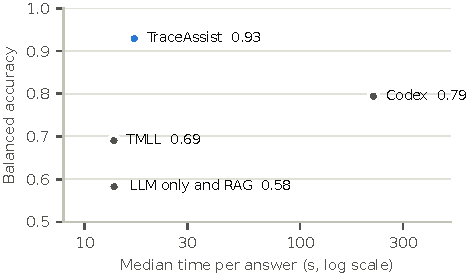
\includegraphics[width=\columnwidth]{time_accuracy}
\Description{Scatter plot of median seconds per answer against balanced accuracy: TraceAssist at 17 s and 0.93, Codex at 219 s and 0.79, TMLL at 14 s and 0.69, LLM only and RAG at 14 s and 0.58.}
\caption{Median time per answer against balanced accuracy (run 1). Times are wall-clock per answer, as recorded by each system's runner; TraceAssist's include building Trace Compass's analyses on the first question about each trace.}
\label{fig:time}
\end{figure}

Fig.~\ref{fig:time} relates time to accuracy.
\sysname's median answer took 17\,s on a desktop workstation; the first question on each trace, which also builds Trace Compass's analyses, took a median of 30\,s. Its answer call used about 27{,}000 input tokens, against 160{,}000--205{,}000 for the LLM-only, RAG and TMLL baselines, because it sends computed findings instead of trace text or every analysis; those baselines answered in a median of 14\,s. \sysname's answer calls cost \$1.41 for all 516 answers; the skills' calls were not logged, so its full cost is somewhat higher. Codex took a median of 219\,s per answer, 13 times \sysname's, running a median of 16 shell commands (11--25 for the middle 80\%) and reading an average of 0.69 million input tokens per answer (92\% from the prompt cache); its 516 answers cost \$9.50. A full bench run of \sysname, asking one question at a time, takes about 3 hours; the LLM-only, RAG and TMLL baselines took 1.2--1.3 hours each (plus 1.3 hours to collect TMLL's evidence), and Codex 17.7 hours with two sessions in parallel.

\subsection{Lessons Learned}
\label{sec:lessons}

We built \sysname against the bench, and each of the fixes below answered a failure the bench exposed. Five lessons generalize beyond our system.

\textbf{1. Measure false alarms, not only answers.} Our prototype evaluation asked only questions whose answer was ``yes'', and \sysname answered all of them correctly. The bench showed that the same system said ``yes'' too often: in a healthy program some thread always finishes last and some wait is always the longest, and the answer writer reported them as problems. Adding sizes to findings (a bottleneck's share of the round, counts of delays by length) and a rule that the answer weigh them against the question's threshold, together with explicit thresholds in the precise wordings, removed most of these false alarms. Negative controls are cheap to build into a test program and are the only way to see this failure.

\textbf{2. Absence of an event is evidence too.} \sysname first answered ``no'' to ``is batch\_server deadlocked?'' on a deadlocked trace. The execution graph records a wait when the thread is woken; a thread that is never woken leaves no wait, so every wait-chain analysis skipped the deadlock. Stuck-wait detection, which reads what each thread is still blocked in at the end of the trace, fixed the hang, deadlock and never-exit cases. The test harness had the same blind spot in reverse: its watchdog's exit woke the blocked threads inside the trace, and the critical path blamed the watchdog.

\textbf{3. Optional evidence fails silently.} \sysname still answers when TMLL is unavailable, only with less evidence. For part of development, every bench answer lacked TMLL's evidence, because its service failed whenever the trace was not open in the Trace Server. Later, a stale experiment index made TMLL allocate 23\,GB and be killed. Neither raised an error in the answers. We now check the services' health around every answer and stamp each answer with a fingerprint of the build and knowledge base, so results from different versions never mix.

\textbf{4. Documentation can leak the answer.} Our first knowledge base, like our prototype's, included a description of \texttt{batch\_server}, standing in for an organization's internal documentation. It named the threads and the lock, and answers cited it instead of the trace. We removed it before the three runs reported here, so their answers rest on the trace alone. Program documentation is valuable in deployment, but an evaluation must separate what the trace shows from what the documents say.

\textbf{5. Put the model where language is needed.} Each LLM call in \sysname makes one narrow decision whose output code checks, and all facts come from code. This kept a small, cheap model usable: the answer writer and two of the three skills run on \texttt{gpt-6-luna}. An agent that computes its own evidence, Codex, took 13 times as long per answer and raised nearly five times as many false alarms (113 against 24).
